\section{Introduction}

The generation of high-quality educational explanations represents a fundamental challenge in natural language processing. Unlike general-purpose conversational tasks, educational rationales must simultaneously satisfy two competing requirements: they must be \textit{logically grounded}, deriving the correct answer through sound deductive steps, and \textit{linguistically fluent}, maintaining natural, readable prose appropriate for a learner audience.

Supervised Fine-Tuning (SFT) on teacher-generated demonstrations has become the standard approach to instilling this capability into LLMs. However, SFT models exhibit a consistent and critical failure mode: while they produce fluent, confident-sounding text, they rarely construct the deductive chain that justifies \textit{why} the correct answer follows from the question context. Empirically, SFT models in our study achieve NLI entailment scores of only 0.05--0.22, indicating that the generated explanation rarely logically implies the ground-truth answer, even when the model ``knows'' the fact.

Reinforcement Learning from Human Feedback (RLHF) and its efficient derivative, Direct Preference Optimization (DPO) \cite{rafailov2023direct}, have sought to move beyond SFT by aligning models to human preferences. Yet these approaches contain a structural flaw when applied to factually demanding tasks: \textbf{the preference signal does not measure logical correctness}. Human annotators, and LLM judges, exhibit a well-documented \textit{verbosity bias}, systematically preferring longer, rhetorically polished responses over concise, logically precise ones \cite{zheng2024judging}. As we demonstrate empirically, GPT-4o-mini awards a 69\% win rate to a verbose SFT baseline over a more logically precise but concise RL-aligned model. DPO trained on such signals therefore reinforces stylistic fluency at the expense of factual grounding, leaving the core alignment gap unaddressed.

A natural remedy is to replace human preference labels with an automated logical metric, specifically, NLI entailment probability. However, optimizing DPO solely against NLI entailment incurs what we term the \textbf{alignment tax}: the model learns to produce short, repetitive snippets that satisfy the NLI scorer but collapse in linguistic coherence. This trade-off between logical soundness and readability represents a fundamental tension that single-dimensional reward signals cannot resolve.

\begin{figure}[h]
\centering
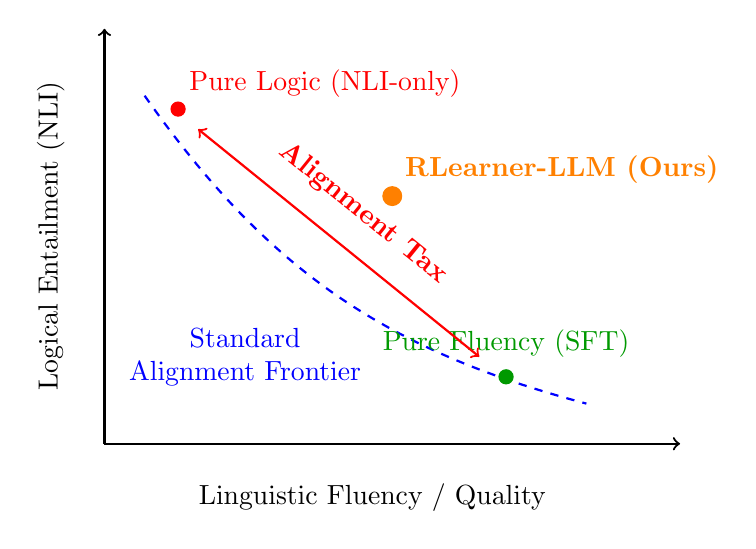
\begin{tikzpicture}[scale=0.85]
% Axes (titles placed clear of the plot to avoid label overlap)
\draw[->, thick] (0,0) -- (8.6,0);
\draw[->, thick] (0,0) -- (0,6.2);
\node[below] at (4.0,-0.45) {Linguistic Fluency / Quality};
\node[rotate=90, above] at (-0.45,3.1) {Logical Entailment (NLI)};

% Standard alignment frontier
\draw[blue, thick, dashed] (0.6,5.2) to[bend right=20] (7.2,0.6);
\node[blue, align=center] at (2.1,1.3) {Standard\\Alignment Frontier};

% Operating points (labels placed inward / above so none run off the axes)
\filldraw[red] (1.1,5.0) circle (3pt) node[above right=0.02cm] {Pure Logic (NLI-only)};
\filldraw[green!60!black] (6.0,1.0) circle (3pt) node[above=0.12cm] {Pure Fluency (SFT)};
\filldraw[orange] (4.3,3.7) circle (4pt) node[above right=0.04cm] {\textbf{RLearner-LLM (Ours)}};

% Alignment-tax trade-off arrow
\draw[<->, red, thick] (1.4,4.7) -- (5.6,1.3) node[pos=0.5, sloped, above=0.2cm] {\textbf{Alignment Tax}};

\end{tikzpicture}
\caption{Conceptual illustration of the \textbf{Alignment Tax}. Standard optimization forces a trade-off between logical grounding and linguistic fluency. RLearner-LLM pushes the Pareto frontier toward the upper-right quadrant through a dual-signal hybrid reward.}
\label{fig:alignment_tax}
\end{figure}

In this paper, we propose \textbf{RLearner-LLM}, a framework that resolves this tension by addressing the root cause directly: the reward signal used to construct preference pairs. Our key insight is that logical grounding and linguistic fluency are \textit{complementary objectives}, not competing ones, and that an automated dual-signal reward combining NLI entailment (for logical soundness) with a verifier score (for pedagogical quality) can construct high-fidelity preference pairs without human annotation, while simultaneously avoiding the degenerate solutions that plague single-signal optimization.

Our contributions are as follows:
\begin{enumerate}
    \item \textbf{Problem diagnosis}: We identify that the root cause of logical misalignment in DPO-trained educational models is not the optimization algorithm itself, but the \textit{reward signal blindspot}: the inability of standard preference signals to measure logical correctness. We provide empirical evidence of verbosity bias in LLM-as-a-judge evaluation that perpetuates this blindspot.
    \item \textbf{Hybrid-DPO framework}: We introduce \textbf{RLearner-LLM}, which automatically constructs preference pairs $\mathcal{D}_{pref}$ using a composite score $H(E_i) = 0.5\cdot S_{\text{NLI}}(E_i) + 0.5\cdot \tilde{S}_{\text{Verifier}}(E_i)$, fusing a DeBERTa-v3 NLI signal with a min-max-normalised verifier LLM score (Eq.~\ref{eq:hybrid_reward}). The dual-signal hybrid eliminates the need for human annotation while overcoming the alignment tax.
    \item \textbf{Cross-architecture validation}: We validate across three base architectures (LLaMA-2-13B, Qwen3-8B, and Gemma 4 E4B-it) and five academic domains (Biology, Medicine, Law), demonstrating up to 6$\times$ NLI improvement over SFT baselines in $11$ of $15$ (architecture, domain) cells, with consistent ACR gains on stronger base models. Gemma 4 E4B-it, a 4.5B-effective-parameter dense model, shows Hybrid-DPO NLI gains in four of five domains (+11.9\% Auckland Law, +32.0\% UK Medicine Y1, +65.6\% Cardiff Biology, +2.4$\times$ UK Medicine Y2), with faster inference across all five and the first single-pass-RL result to surpass the iterative ILearner-LLM (K=5) baseline on Auckland Law NLI. Our Qwen3-8B model further wins $95\%$ of blind pairwise comparisons against its own SFT baseline; on the same judge it loses $95\%$ to GPT-4o-mini's longer outputs, replicating the verbosity bias on a frontier comparator and motivating logic-aware automatic metrics over LLM-as-a-judge for knowledge-intensive generation.
    \item \textbf{Robustness to question-quality filtering}: Using the full PeerWise answer-submission logs, we show the gains survive a \textit{strict-discriminator} filter that keeps only questions whose author key matches the \emph{modal student answer}: across three architectures and two corpora, answer-coverage improves in all six (architecture, corpus) cells and NLI in four of six, reproducing the per-architecture pattern of the main results (Appendix~\ref{sec:tierc_appendix}).
    \item \textbf{Independent validation and a step toward reasoning}: An out-of-training held-out NLI scorer (DeBERTa-v3-large) reproduces the improvement direction in $12$ of $15$ main cells, evidence against reward-hacking of the training scorer. Going beyond entailment, we build a pairwise reasoning-quality reward and, using a length-normalised objective, obtain a compact model whose explanations two independent judges prefer over the SFT baseline ($70$--$72\%$ of non-tied pairs) \emph{at matched output length}, indicating the gain is genuine reasoning quality rather than verbosity (\S\ref{sec:reasoning-reward}, Appendix~\ref{sec:reasoning_appendix}).
\end{enumerate}
